\documentclass{beamer}
\usetheme{intridea}
\usepackage{listings}

\title{Intro to {\TeX} and {\LaTeX}}
\subtitle{The Programming Language for Creating Beautiful Documents}
\author{John McAvoy}
\institute{A-Team Workshop}
\date{February 8, 2019}

\begin{document}

\frame{\titlepage}

%\begin{frame}
%\frametitle{Table of Contents}
%\tableofcontents
%\end{frame}

\begin{frame}
  \frametitle{What is {\TeX} and {\LaTeX}?}

  \begin{itemize}
    \item \textbf{\TeX} (= tau epsilon chi, and pronounced similar to "blecch",
      not to the state known for `Tex-Mex' chili) is a computer language
      designed by Donald Knuth for use in typesetting; in particular, for
      typesetting math and other technical (from Greek "techne" = art/craft, the
      stem of 'technology') material. It was t takes a "plain" text file and
      converts it into a high-quality document for printing or on-screen
      viewing.\cite{tug} \cite{wikibooks}

    \item \textbf{\LaTeX} is a macro system built on top of TeX that aims
      to simplify its use and automate many common formatting tasks. It is the
      de-facto standard for academic journals and books, and provides some of
      the best typography free software has to offer. \cite{wikibooks}

  \end{itemize}
\end{frame}

\begin{frame}
  \frametitle{What is {\TeX}/{\LaTeX} Used For?}
  \begin{itemize}
    \item \textbf{Making Documents With Complex Formats}
    \item \textbf{Technical Papers}
      \begin{itemize}
        \item Research Papers
        \item IEEE Documents
      \end{itemize}

    \item \textbf{Literally And Written Medium}
      \begin{itemize}
        \item Essays
        \item Novels
        \item Journal Articles
        \item Lab Reports
        \item Memos
        \item Slideshows?
        \item And so much more!
      \end{itemize}
  \end{itemize}
\end{frame}

\begin{frame}
  \frametitle{What Does {\TeX} Look Like?}
  \begin{itemize}
    \item
      \href{http://mirror.utexas.edu/ctan/macros/latex/contrib/IEEEtran/IEEEtran_HOWTO.pdf}{IEEETran
        (the {\LaTeX} format guide that all articles published by IEEE must use)}
    \item \href{https://ieeexplore.ieee.org/stamp/stamp.jsp?tp=&arnumber=6740844}{Internet of Things for Smart Cities}
    \item
      \href{../../example/sample_docs/emags_lab/output/lab_05.pdf}{Lab Report Example}
    \item
      \href{../../examples/sample_docs/signals_lab/report/output/final_project.pdf}{Lab
        Repo../rt Example With Code Snippets}
    \item
      \href{../../examples/sample_docs/resume/output/cv_4.pdf}{Resume Example}
    \item
      \href{../../examples/sample_docs/abet_documentation/docs/output/doc.pdf}{Documentation Example}
    \item
      \href{../../examples/sample_docs/abet_instruction_manual/instructions/output/manual.pdf}{User
        Manual Example}
    \item
      \href{../../examples/sample_docs/code_documentation/report/output/calculator.pdf}{Code
        Documentation}
    \item \href{https://www.overleaf.com/latex/templates}{Tons of More Template
        to Get You Started}

  \end{itemize}
\end{frame}

\begin{frame}
  \frametitle{{\LaTeX} vs Word}
  \begin{figure}
    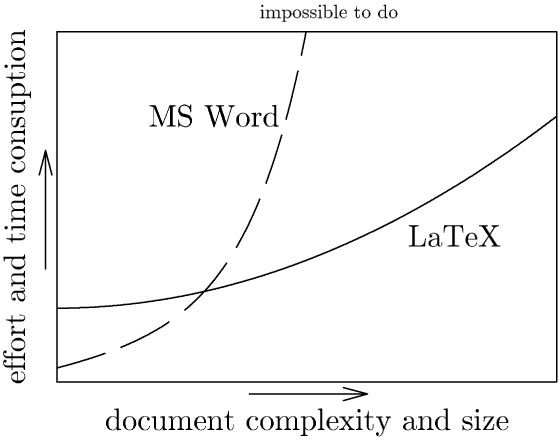
\includegraphics[width=0.70\framewidth]{./img/latex_vs_word_graph.png}
    \caption{Effort and Time Comparison: Word vs {\LaTeX} \cite{pintric}}
  \end{figure}
\end{frame}

\begin{frame}
  \frametitle{How to Start Writing {\TeX} Documents}
  \begin{itemize}
    \item \textbf{Option I: Use \href{overleaf.com}{Overleaf}}
      \begin{enumerate}
        \item Make a free, personal overleaf account
        \item Make your first {\TeX} project
        \item That's basically it, you can start writing {\TeX}
      \end{enumerate}
    \item \textbf{Option II: Write {\TeX} Documents Locally}
      \begin{enumerate}
        \item \textbf{Download a {\TeX} Language Compiler and a TeX Package Manager}
          \begin{itemize}
            \item Windows:
              \href{http://ctan.math.illinois.edu/systems/windows/protext/}{proTeXt}
            \item MacOS:
              \href{https://www.tug.org/mactex/mactex-download.html}{MacTeX}
            \item Unix/GNU/Linux:
              \href{https://tug.org/texlive/acquire-netinstall.html}{TeX Live}
          \end{itemize}
        \item Configure your favorite text editor or IDE to support {\TeX}
          syntax highlighting, a {\TeX} IDE may already be included in MacTeX and TeX
          Live)
        \item Compile your {\TeX} and that's it.
      \end{enumerate}
  \end{itemize}
\end{frame}

\begin{frame}
  \frametitle{Pros and Cons}

  \begin{itemize}
    \item \textbf{Option I: Use \href{overleaf.com}{Overleaf}}
      \begin{itemize}
        \item \textbf{Pros:}
          \begin{enumerate}
            \item It's the fastest way to learn how to make documents in a
              {\TeX} environment
            \item Overleaf has all of the {\TeX} packages you will ever need so
              you don't have to bother with installing packages
            \item You get access to a plethora of pre-made templates
            \item It's essentially Google Docs for {\LaTeX}, you can collaborate
              with friends on reports
            \item Overleaf has live rendering of your document so you can see
              what your document looks like as you write {\TeX} code
            \item Overleaf has error checking and basic debugging that is decent
          \end{enumerate}
        \item \textbf{Cons:}
          \begin{enumerate}
            \item It's a cloud-based service so you have to have an internet
              connection
            \item You have to upload files that you reference in your {\TeX},
              (e.g. images, code snippets)
            \item Some features like collaboration cost a monthly fee
          \end{enumerate}
      \end{itemize}
  \end{itemize}
\end{frame}
\begin{frame}
  \frametitle{Pros and Cons}
  \begin{itemize}
    \item \textbf{Option II: Write {\TeX} Documents Locally}
      \begin{itemize}
        \item \textbf{Pros:}
          \begin{enumerate}
            \item You can write {\TeX} anywhere, no internet required
            \item You can use your favorite text editor
            \item The fastest way to write {\TeX} documents
            \item There are many {\TeX} IDE's that usually bundle a {\TeX}
              compiler, a {\TeX} package manager, and a text editor
            \item You can reference local files (e.g. images, code) and when you
              change them, you just have to recompile and all changes are
              updated in you document
            \item 100\% free
          \end{enumerate}
        \item \textbf{Cons:}
          \begin{enumerate}
            \item Need to download stuff
            \item Have to install {\TeX} packages yourself
            \item Requires a little bit of configuration at first
          \end{enumerate}
      \end{itemize}
  \end{itemize}
\end{frame}

\begin{frame}
  \frametitle{Where to Get Started}
  \begin{itemize}
    \item
      \textbf{\href{https://www.overleaf.com/learn/latex/Main_Page}{Overleaf's
          {\LaTeX} Tutorials}} are excellent
    \item All of the {\TeX} source to make this presentation, as well as some
      {\TeX} documents I've created can be found on
      \textbf{\href{https://github.com/JOHNeMac36/tex_workshop}{GitHub}}
  \end{itemize}
\end{frame}

\begin{frame}
  \frametitle{Bib{\TeX}}
\end{frame}


\begin{frame}
  \frametitle{Works Cited}
  \begin{thebibliography}{9}
    \bibitem{tug} {\TeX} User Group \url{http://tug.org}
    \bibitem{wikibooks} WikiBooks:{\LaTeX} \url{https://en.wikibooks.org/wiki/LaTeX}
    \bibitem{pintric} Pintric \url{http://www.pinteric.com/pic/miktex.gif}
  \end{thebibliography}
\end{frame}

  \end{document}
